\section{ПОТРЕБНОСТЬ В РАЗРАБОТКЕ}

\subsection{Анализ текущих методов заполнения и хранения карт вызова}

В настоящее время, при вызове скорой помощи, медики используют методические пособия и бланки карт вызова, которые хранятся в объемной папке.

Метод заполнения карт вызова имеет свои особенности. В зависимости от состояния пациента, медики заполняют различные разделы карты, начиная от основной информации о пациенте и заканчивая деталями о его состоянии, симптомах и проведенных медицинских процедурах.

Для правильного заполнения карт вызова медицинскими работниками требуется знание определенных протоколов и стандартов. Для этого они обычно имеют с собой несколько методических пособий, содержащих инструкции по заполнению различных разделов карты вызова в зависимости от состояния пациента. Это усложняет процесс и требует дополнительного времени и усилий. Помимо этого, медицинские работники заполняют карты вызова в процессе осмотра пациента. Это требует их присутствия и внимания к пациенту, а также необходимости записывать информацию вручную.

Хранение карт вызова также имеет свои особенности. Обычно эти документы хранятся в специальных папках или ящиках машины скорой помощи, доступных только медицинским работникам, которые после окончания смены передаются отделению в медицинском учреждении для формирования отчетности. Это создает дополнительный вес и занимает место в машине скорой помощи, а также создаёт проблемы с доступом к предыдущим записям и усложняет поиск и извлечение информации о конкретных пациентах или случаях. 

Однако, существуют и недостатки текущих методов заполнения и хранения карт вызова. Например, при использовании бумажных бланков возможны ошибки в заполнении или потеря документов. Кроме того, доступ к картам вызова может быть ограничен, что затрудняет своевременное и эффективное оказание медицинской помощи.

В связи с этим, возникает потребность в новых технологиях, которые позволят ускорить процесс заполнения карт вызова, уменьшить количество ошибок и обеспечить безопасное хранение этих документов. Таким образом разработка web-сервиса, позволяющего заполнять карты вызова в электронной форме, представляет собой актуальное и необходимое решение для улучшения и оптимизации процесса работы медицинских работников из отделения неотложной медицинской помощи.

В целом, анализ текущих методов заполнения и хранения карт вызова показал, что они имеют свои преимущества и недостатки. Но в современном мире, где ценится скорость и качество медицинской помощи, возникает потребность в новых технологиях, которые помогут повысить эффективность работы медицинских работников и обеспечить быстрое и точное оказание помощи пациентам.

\subsection{Описание проблем и ограничений существующих решений}

Анализируя существующие решения, такие как сайт-прототип заполнения карт вызова onmp.ru, представленный на рисунке~\ref{fig:onmp-prototype},

\begin{figure}
  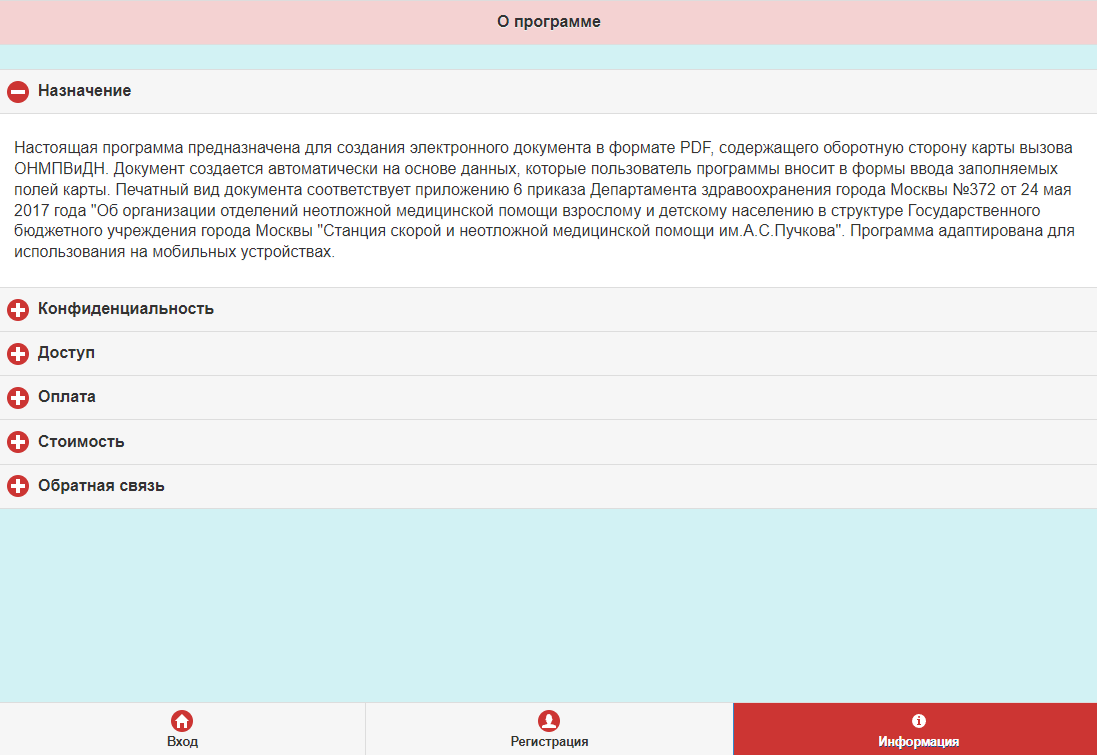
\includegraphics[scale=0.5]{styles/diploma/inc/onmp-prototype.png}
  \caption{Сайт-прототип onmp.ru}
  \label{fig:onmp-prototype}
\end{figure}
можно выделить несколько проблем и ограничений, которые ограничивают его удобство использования и эффективность:

Язык программирования PHP: Использование PHP для разработки сайта может ограничивать его гибкость и масштабируемость. PHP является языком серверной разработки, и его использование может усложнить внесение изменений и расширение функциональности клиентской части.

Неудобный UX-дизайн: Отсутствие интуитивного и удобного UX-дизайна на сайте может создавать сложности при навигации между разделами, а также затруднять быстрый доступ к нужной информации. Неочевидные переходы и отсутствие удобной навигации могут снижать эффективность работы мед.работников и увеличивать время заполнения карт вызова.

Отсутствие промежуточного сохранения: Наличие функции промежуточного сохранения карт вызова является важным аспектом для удобства пользователей. Отсутствие такой функции на сайте может приводить к потере данных в случае прерывания работы или случайного закрытия страницы.

Ограниченные возможности навигации по карте: Отсутствие быстрой навигации по карте вызова может затруднять поиск и редактирование определенных разделов или полей, особенно в случае больших и сложных карт.

Учитывая эти проблемы и ограничения существующего решения, разработка нового web-сервиса для заполнения карт вызова с использованием React.js имеет потенциал для устранения данных проблем и предоставления более удобного и эффективного инструмента для медицинских работников из отделения неотложной помощи.

\subsection{Обзор преимуществ перехода на электронную форму заполнения карт вызова}

Переход на электронную форму заполнения и хранения карт вызова имеет несколько преимуществ. 

\begin{itemize}
    \item Использование электронной формы позволяет существенно сократить потребление бумаги и уменьшить негативное влияние на окружающую среду. Это способствует экологической устойчивости и снижению расходов на закупку и хранение бумажных материалов.
    \item Электронная форма позволяет быстро и удобно заполнять карты вызова, что ведет к повышению эффективности работы медицинских работников. Заполнение осуществляется путем выбора и ввода данных в соответствующие поля, что сокращает время, затрачиваемое на ручное заполнение бумажных форм.
    \item Электронная форма обеспечивает легкий доступ к заполненным картам вызова из любого места с подключением к Интернету. Это позволяет медицинскому персоналу быстро получать необходимую информацию о пациентах, это особенно полезно для медицинских работников, которые находятся в пути, например, в машине скорой помощи. Они могут легко получить доступ к системе и заполнить карты вызова на своих устройствах. Также электронна форма облегчает анализ и обработку данных для статистической отчетности и исследований. Помимо этого, медицинский персонал может получить доступ к предыдущим записям о состоянии пациента и процедурах, которые ему проводились, что помогает улучшить качество медицинской помощи и сделать более точный диагноз.
    \item При использовании электронной формы можно внедрить функциональность автоматического заполнения и проверки данных. Например, система может предложить автозаполнение некоторых полей на основе предыдущих записей или данных из других систем, а также проводить проверку на наличие ошибок или недостаточных данных.
    \item Электронные карты вызова могут быть сохранены в централизованной базе данных, что облегчает их архивирование и поиск. Можно использовать различные фильтры и категории для организации и классификации карт по статусу (готовые, незавершенные, архив) или другим параметрам, упрощая их управление и обработку.
    \item В электронной форме можно создавать шаблоны часто используемых или стандартных карт вызова. Это позволяет медицинскому персоналу быстро заполнять карты, используя предварительно сохраненные данные, что повышает производительность и снижает вероятность ошибок.
\end{itemize}

Переход на электронную форму заполнения карт вызова значительно сокращает бумажную работу, повышает эффективность и точность процесса заполнения, улучшает доступность и хранение данных, а также облегчает анализ и управление информацией. Это современный и инновационный подход, который может значительно улучшить работу мед.работников и повысить качество оказываемой медицинской помощи.
